% !TEX root =  paper.tex


\section{Proposed Approach}
\label{section:approach}


\Cref{fig:approach-diagram} shows an overview of our proposed approach
to automatically generate modularized reusable UI components
from mockups.
The approach begins by retrieving the DOM of the web app's mockup. 
Next, a visual abstraction is performed to generate a normalized and abstract representation of the web app's UI layout.
This transforms the mockup into a set of {\VizElem}s ({\VE}s) on which further analysis is conducted. 
The approach then performs a dynamic grouping  of {\VizElem}s,
to identify subtrees
which correspond to potential instances of a UI component. 
This grouping is used in the next step, where an unsupervised machine learning technique applied on the 
potential UI component instances identifies UI components.
Finally, the actual code for the UI components is generated by refactoring the original \html code.

\begin{figure}
    \centering
    \includegraphics[width=0.75\linewidth]{maintainability/figures/approach-diagram}
    \caption{Overview of the proposed approach.} 
    \label{fig:approach-diagram}
\end{figure} 


In the following subsections, we describe each step of the proposed approach and illustrate some of their major components and analysis procedures. 

\subsection{Definitions}
Before we proceed to describe the details of the proposed approach, we begin by declaring a few important definitions that are used throughout the chapter.
\begin{defn}[\textbf{UI Component}]
A UI component $c_E=\langle n, N \rangle$ 
for a repeated group of UI element trees $E$ in a web application
is a tree structure rooted at $n \in N$, where $N= T \cup P$ is a set of abstract user interface elements.
The component includes the \emph{template} $T$ and the \emph{placeholders} $P$.
The template of the UI component denotes the nodes which do not change wherever the component is used (i.e., \emph{instantiated}),
while the placeholders captures the changed nodes, whether partially or fully changed, as explained in \Cref{sec:ui-comp-gen}.
\end{defn} 
In this chapter, we use the terms \textit{UI component} and \textit{component} interchangeably.


\begin{defn}[\textbf{Component Instance}]
A component instance $i=\langle c_E, f \rangle$ is a concrete and specific instantiation of a UI component $c_E$. 
Component instances share the template part with other instances of the same component, 
but differ in the placeholder parts.
The function $f: P \rightarrow V$ assigns values $v \in V$ to the placeholders $p \in P$ of $c_E$.
\end{defn}

\begin{defn}[\textbf{Potential Instance}]
A potential instance is a subtree of the \dom 
constructed for a web application's user interface,
representing a concrete UI element tree 
that is \emph{likely} to form a component instance, but may not be so. 
\end{defn}

Potential instances are processed at multiple stages of the proposed approach 
until they are either discarded or associated with a component.


\subsection{Visual UI Normalization}
In the first step of the approach, we take as input the DOM of the mockup after it is loaded and rendered in a browser,
and perform a \emph{visual normalization} that transforms the DOM into a set of \emph{{\VizElem}s}.
The goal of this step is to normalize the visual presentation of a web user interface into a set of abstract elements 
that signify the salient features of the page from a visual perspective, which may represent potential component instances.
The intuition behind this is that normalization and abstraction can be helpful to achieve our goal of detecting reusable patterns, since the exact and minute details are less relevant when identifying repeated regions of a web page. 
Furthermore, component instances are generally different from each other in some aspects, while they still have similar overall visual appearance. 
This normalization step enables obtaining a big picture to identify these potential similarities.% between different instances.

The visual normalization is achieved as follows.
First, we extract from the DOM a set of nodes that represent visual content of the UI, and we refer to each of these as \emph{{\VizElem}s}.
We define two main types of {\VizElem}s: textual and graphical (image).
The extraction of text content is achieved by traversing text nodes of the DOM. More specifically:
%\begin{align}
%VE_{T} \coloneqq \{ node \in DOM \!\, : \, & node.type=\code{\#TEXT} \nonumber \\
%                       \lor \, & node.tag=\code{input} \}
%\end{align}
\begin{align}
\Gamma_{T} \coloneqq \{ E(node) : \ & node \in DOM_R \!\, 			\land \,  & node.hasTextContent \}
\end{align}
where $\Gamma_{T}$ is the set of all visual elements that represent text in the UI, $DOM_R$ is the rendered DOM in the web browser, and $E(node)$ maps the node to the corresponding element. 
%\davood{visual element?}
The predicate $hasTextContent$ examines whether there is a text associated with the node, 
and covers two possibilities: non-empty nodes of type \code{\#TEXT}, representing string literals in $DOM_R$, 
and nodes of \code{input} elements that have an associated text value (e.g., buttons or lists).
Subsequently, we perform another extraction for image content. We define this as follows:

%\begin{align}
%VE_{I} \coloneqq \{ & node \in DOM \!\, : \, node.tag=\code{img} \nonumber \\
%                       \lor \, & node.hasBackgroundImage \}
%\end{align}
\begin{align}
\Gamma_{I} \coloneqq \{ E(node) : \ & node \in DOM_R \!\, 		\land \, & node.hasImageContent \}
\end{align}
where $\Gamma_{I}$ is the set of all visual elements that represent images. As in the previous case, the predicate $hasImageContent$ examines if there is an image associated with the node. This again has two possibilities: nodes of \code{<img>} elements and non-img nodes with a non-null background image attribute. 

Subsequently, we use the set of all {\VizElem}s to construct the normalized UI: 
\begin{align}
\mathrm{UI}_N = V\!\left( \Gamma_I \cup \Gamma_T \right)
\end{align}
where $\mathrm{UI}_N$ is the resultant normalized UI and $V$ is a visual projection operation that generates an image from the union of visual elements. This is achieved as follows. First, we begin by collecting the final \emph{computed} properties of each element,
when rendered in the web browser. These properties represent the final state of elements after the propagation of all changes and events. The properties we collect are the size, location, and z-orders of these elements. Next, we assign different colors to each class of {\VizElem}s.
We assign green for elements in $\Gamma_{T}$, and blue for elements in $\Gamma_{I}$.
While any arbitrary colors could have been chosen, we chose these two colors in order to facilitate faster visual analysis in subsequent steps, since these two  are typically represented in separate color channels.
\Cref{fig:example-normalization} illustrates an example of the output generated from this visual normalization step.
As can be observed, the minute details of the page are abstracted away while the main and essential structure of the UI is accentuated. 

\begin{figure}
    \centering
    \includegraphics[height=3.5cm,width=0.40\textwidth, clip, trim={0 0cm 0 0cm}]{maintainability/figures/example-normalization}
    \caption{The result of the visual UI normalization stage (as applied to the motivating example of \Cref{fig:motivating-example}). Best viewed on a color display.}
    \label{fig:example-normalization}
\end{figure} 

\subsection{Potential Instance Identification}
The result of the previous step consists of only a set of {\VizElem}s.
These {\VizElem}s on their own do not \emph{necessarily} represent reusable repetitive UI patterns. 
The goal of this step is to transform the set of individual {\VizElem}s into a set of \emph{potential} reusable UI component instances.
A potential instance is a region of the UI that has been determined to be likely repeated somewhere else in the UI. That is, it is 
a region where, using all of the aforementioned steps, the 
initial analysis have indicated that this instance would likely be a good candidate to be combined with other repetitions and refactored 
into a single component. These potential component instances will be further checked and analyzed in the subsequent steps in order to generate a final set of components.

Identifying potential component instances can be an intricate decision since there are multiple levels of hierarchy that can be considered.
For example, consider group \circled{A} in \Cref{fig:motivating-example}.
Notice how the icons in that group would constitute repeated elements.
The same is true for the text labels under the icons.
Yet another repetition pattern is taking the icon and text as one component that is repeated multiple times. 
Accordingly, in order to identify potential component instances, we propose an approach that aims to maximize two complementary aspects, namely, 
the number of repetitions of a component,
and the amount of repetitions encapsulated \emph{within} each component instance (i.e.,~repetitions of the \emph{same} potential instances).
We refer to this combination of aspects as the \emph{modularization potential}, where a high value of modularization potential indicates a potentially more reusable UI component.
Our goal is therefore to utilize this modularization potential to optimize a set of potential instances, $\Psi$:
% capture these aspects in a quantitative manner and optimize for the \emph{maximal modularization component set}, $MMCS$:
%\begin{equation} \label{eqn:MMCS}
%\Psi \coloneqq \argmax_{C} \prod_{c_i \in C} \big\lvert \{VE_T \cup VE_I  : VE_T, VE_I \in c_i\} \big\rvert
%\end{equation}
\begin{equation} \label{eqn:MMCS}
\Psi \coloneqq \argmax_{C} \prod_{c_i \in C} \big\lvert \{c_i(\gamma_T, \gamma_I) : \gamma_T, \gamma_I \subset \mathrm{UI}_N\} \big\rvert
\end{equation}
where $C$ is the set of all component instances, $c_i$ is a potential instance, and the optimized function is the modularization potential.
This optimization yields a global optimum set of potential instances between two extremes.
At one end of the spectrum,
each {\VizElem} represents a component of its own.
This yields a sub-optimal component set that has low modularization potential because of a lack of repetitions.
For this case, the modularization potential in \cref{eqn:MMCS} yields a score of 1 since each component encapsulates only a single element.
At the other end of the spectrum,
one might theoretically consider the \emph{entire} collection of {\VizElem}s to represent a single component that is repeated only once.
This results in a score equal to $N$, the number of total {\VizElem}s, in \cref{eqn:MMCS}.
$\Psi$, on the other hand, represents a global optimum between the aforementioned two extremes. $\Psi$ captures a set of potential component instances that aims for \emph{both} a large number of components, and for an instance that in itself has a large number of UI repetitions.
The subsequent steps of the approach will therefore only use $\Psi$ for further analyses and final generation of components.

We now describe the implementation for generating $\Psi$. \Cref{fig:instance-potential-identification} shows an illustration of this process.
First, we obtain DOM locators (e.g., {\xpath} expressions) for each of the {\VizElem}s. Next, starting from these locators as leaf nodes, we iteratively build a tree from the bottom up (as shown in \Cref{fig:instance-potential-identification}), adding the DOM parent of every tree node with each iteration.
At each iteration, we calculate the modularizaton potential of \cref{eqn:MMCS}, with every node's subtree representing a potential instance $c_i$. 
The potential instances are illustrated using the red outlines in \Cref{fig:instance-potential-identification}. Note how at the very first iteration, each potential instance is simply the \VizElem~itself. In the next iteration, the potential instances grow larger to include more {\VizElem}s as shown by the larger red outlines at iteration 1.
Finally, the iteration that yields the maximal modularization is  reported as the $\Psi$ set and passed to the subsequent stage.

\begin{figure}
    \centering
    
\includegraphics[width=0.9\linewidth]{maintainability/figures/potential-component-identification}
    \caption{Illustration of the potential instance identification stage. Each iteration considers a different group of potential instances before selecting an optimum set.}
    \label{fig:instance-potential-identification}
\end{figure} 

\subsection{Unsupervised Visual Matching}
The output of the previous step is a set of \emph{potential} component instances that maximizes the modularization potential out of many alternative sets of instances.
However, these are only \emph{potential} instances that may or may not actually belong to a component.
In other words, there is still no information as to which subgroup of potential instances do indeed belong together and constitute a reusable component,
versus other potential instances that are simply visual elements that do not represent repetitive reusable components.
In this stage, we process the set of \emph{potential} component instances and reduce it into a final set of components. 

In order to create the final components,
we propose an approach that visually examines potential instances and combines them into components via unsupervised machine learning.
The intuition behind adopting this approach is that if potential instances match with other potential instances,
the ``potential'' qualifier can be dropped from these instances and they would be recognized as constituting a component together.
In this approach, we use a clustering mechanism to create components in order to facilitate robust matching of potential instances.

We now describe the details of the process. First, we obtain the screenshot image of the {\VizElem}s per potential instance. This results in one image (containing all {\VizElem}s) for each potential instance. Next, for each potential instance image, we extract a feature vector. We compute the feature vector using a \emph{vectorized pixel histogram}, which is a process that captures a summary of the overall content in the instance image. However, unlike typical approaches from the machine vision literature~\cite{lopes2010automatic, liu2010image} where a binning parameter (a parameter for categorizing pixels) is required, we generate the vectorized histogram without requiring this parameter. Instead, due to the nature of visual normalization that we have proposed, only two categories need to be considered: one for text visual elements, and another for image visual elements. Therefore, we finally end up with a feature vector for each potential instance. Subsequently, we compute the cosine distance between each pair $\mathbf{I}_i$, $\mathbf{I}_j$ of potential instances:
\begin{equation} \label{eqn:cosdist}
D_{i,j} = 1 - \frac{\mathbf{I}_i \cdot \mathbf{I}_j}{ \lVert \mathbf{I}_i \rVert \lVert \mathbf{I}_j \rVert }
\end{equation}

Next, we perform an unsupervised clustering process. The selection of an appropriate clustering is of paramount importance due to a couple of challenges. First, the clustering can be challenging due to the wide range of possibilities of arrangements and structures of component instances. In other words, there is potentially a large range of \emph{inter-} and \emph{intra-}component variations. 
This makes it difficult to use hierarchical clustering, for instance, due to its very high sensitivity to outliers and therefore would be a poor choice for handling large component variations, and also due to its high dependence on order of data, which can make it less effective for detecting instances far way from each other. Furthermore, performing a cut on the clustered hierarchies often requires specifying the number of clusters or some other parameter, which can be difficult and brittle to specify. Density-based algorithms (e.g., DBSCAN) would not be effective either, as they would have difficulty handling the \emph{variable} densities present between potential clusters of instances. Accordingly, we opted for a technique that can be flexible enough to correctly identify such variations and be able to better recognize the final components. To do this, we select a method that performs variable-density clustering with a hierarchy of densities \cite{campello2013density}. The hierarchy of variable-densities allows the method to automatically detect stable clusters in a parameter-free fashion. More importantly, the method is built to handle varying-densities, which becomes very important when handling the potentially large range of inter- and intra-component variations.
 
Once the components have been identified through unsupervised visual matching,
we extract the corresponding locator in the DOM (e.g., {\xpath}s) per instance.
The final result is a superset of component instance locator sets.
This superset is passed on to the next step in order to combine the component instances into final components.


\subsection{UI Component Generation}
\label{sec:ui-comp-gen}
% !TEX root =  paper.tex
We propose an algorithm that unifies the UI component instances 
identified in the previous steps
into a component
implemented using a web framework (e.g., \react, \angular, \html Web Components~\cite{MDN:2017:WebComponents}).
However, instead of directly generating the framework-specific code for components,
we opt for constructing an \textit{intermediate model}
that effectively represents components at a higher level of abstraction.
This allows building different \textit{translation strategies}
for generating the actual code 
for different frameworks from the same model,
with the added benefit of remaining agnostic 
to the specific details of a particular framework. 
Our implementation supports the \react~\cite{React} translation strategy,
 which is the preferred framework for a significant number of developers in practice~\cite{StateOfJS:WebPlatformTests, StackOverflow:2017:Survey}.
We first define the terms used in this step.

\begin{defn}[\textbf{\mappedset}]
	\label{definition:mapped-nodes-set}
	Let $T = \{t_1 \ldots t_n\}$ be the list of \dom subtrees for $n$ instances
	of a UI component identified by the previous phases of the approach.
	%These subtrees are rooted at the \dom nodes located by the {\xpath}s 
	%returned by the previous phase.
    A set $D = \{d_1 \in t_1, d_2 \in t_2\ldots d_n \in t_n\}$ of \dom nodes corresponding to $T$
	is a \mappedset,
	when every pair $(d_i, d_j)$ of \dom nodes 
	belonging to $D$ are \textbf{mapping}.
\end{defn}

\begin{defn}[\textbf{Mapping}]
	Two \dom nodes $d_i$ and $d_j$
	are mapping (denoted as $d_i \leftrightsquigarrow d_j$) when:
	\begin{itemize}[leftmargin=*]
	\item Both $d_i$ and $d_j$ are root nodes of their trees, or 
	\item $d_i$ and $d_j$ are not root nodes, and
	\begin{itemize}[leftmargin=*]
		\item $d_i.parent.tag = d_j.parent.tag$, and
		\item $d_i.parent \leftrightsquigarrow d_j.parent$, and
		\item $d_i$ and $d_j$ have the same child index 
		(e.g., they are both the first child of their parents).
	\end{itemize}

	\end{itemize}
\end{defn}

\begin{defn}[\textbf{\model}]
	The \model is a rooted, ordered tree
	in which each node corresponds to a \mappedset.
	The hierarchy of this tree follows the mapping \dom nodes' hierarchy.
\end{defn}


\header{Example} \Cref{fig:intermediate-model-sample-dom-subtrees}(a) 
depicts the \html code snippets 
corresponding to two identified UI component instances.
%(the visual output is omitted due to space limitations).
The corresponding \dom subtrees,
and the constructed \model for these subtrees 
are respectively shown in \Cref{fig:intermediate-model-sample-dom-subtrees}(b) and (c).
The connected \dom nodes with dotted arrows form {\mappedset}s.
Notice that non-mapping \dom nodes do not form a node in the intermediate model.
This model can be translated to a \react-like component
similar to what is shown in \Cref{fig:intermediate-model-sample-dom-subtrees}(d).
Finally, the generated component is instantiated two times in the refactored \html code
to replace the originally-repeated \dom nodes.
The calls to the component can look like what is shown in \Cref{fig:intermediate-model-sample-dom-subtrees}(e).

\begin{figure}
    \centering
    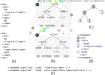
\includegraphics[width=0.70\textwidth]{maintainability/figures/intermediate-model}
    \caption{
    	(a) Initial \html code fragments.
     	(b) Corresponding \dom subtrees.
     	(c) The constructed \model.
     	(d) The final generated UI component.
     	(e) The \textit{calls} to the generated UI component.}
    \label{fig:intermediate-model-sample-dom-subtrees}
\end{figure} 

When generating the actual framework code,
each model node results into a \dom node in the framework component
(as depicted in \Cref{fig:intermediate-model-sample-dom-subtrees}(d)),
which essentially \textit{unify} the nodes in the \mappedset
to remove duplication.
There are three possibilities for framework component \dom nodes:

\begin{itemize}[leftmargin=*]

	\item When all pairs of \dom nodes in a \mappedset have the same tag and identical attribute values,
	they can be unified in one \dom node of the same tag.
	For example, the two \code{<div>} nodes in \Cref{fig:intermediate-model-sample-dom-subtrees}
	corresponding to model node \circled{1}
	form a \code{<div>} node in the component.
	
	\item A pair of \dom nodes in a \mappedset which have different tag names
	cannot be unified into one \dom node in the component
	(e.g., \code{<span>} and \code{<div>}
	corresponding to model node \circled{5} in \Cref{fig:intermediate-model-sample-dom-subtrees}).
	Similar is two text nodes with different content
	(e.g., the \code{foo} and \code{bar} corresponding to the model node \circled{3} in \Cref{fig:intermediate-model-sample-dom-subtrees}).
	In such cases, the \dom nodes (and the whole subtree rooted at them) should be \textit{hard-parameterized} in the resulting component,
	i.e., a \textit{placeholder} should be created.
	The original parameterized \dom nodes are later passed as \textit{arguments} when instantiating the component
	to recreate the original \dom hierarchy.
	
	\item A pair of \dom nodes in a \mappedset that have the same tag name but
	different values for one of their attributes
	might be unifiable into a \dom node 
	via \textit{soft parameterization},
	where the differing attribute values are parameterized
	(e.g., the \code{<img>} tags corresponding to model node \circled{4}
	in \Cref{fig:intermediate-model-sample-dom-subtrees},
	with parameterized \code{src} attribute values).
	This can be done only if the used framework supports parameterizing attribute values.
	Otherwise, the parameterization should be done as if it was a hard parameterization.

\end{itemize}

\header{The intermediate model construction and refactoring algorithm}
The inputs of \Cref{algorithm:refactoring} are the original mockup \html, 
the list of component instance \dom subtrees,
and the translation strategy.
The output is the refactored \html wherein duplication is removed using the UI components.

\begin{algorithm}
	\fontsize{7.5pt}{9pt}\selectfont
	%\linespread{1}\selectfont
	\caption{\model Generation}
	\label{algorithm:refactoring}
	% !TEX root =  paper.tex

\begin{algorithmic}[1]

\renewcommand{\algorithmicrequire}{\textbf{Input:}}
\renewcommand{\algorithmicensure}{\textbf{Output:}}

\Require \par ~ The original \dom of the mockup ($DOM_{original}$),
UI component instances \dom subtrees ($subtrees$), 
UI component translation strategy ($strategy$)

\Ensure The new \dom after refactoring ($DOM_{refactored}$)


\State $model \gets \Call{ConstructEmptyIntermediateModel}{{}}$ \label{algoline:ui-component-empty-model}
\State $coveredNodes \gets \varnothing$ \label{algoline:ui-component-covered-nodes-init}
\State $templateTree \gets \Call{getSmallestTree}{subtrees}$ \label{algoline:ui-component-template-tree}
\State $templateNodes \gets \Call{BFS}{templateTree}$
\For{$templateNode \in templateNodes \setminus coveredNodes$} \label{algoline:ui-component-main-loop-start}
	\State $coveredNodes \gets coveredNodes \cup \{ templateNode \}$
	\State $mappedNodes \gets \Call{getMappedNodesSet}{templateNode, subtrees}$\label{algoline:ui-component-mapped-nodes-set}
	\State $parameterization \gets \code{NULL}$
	\For{$currentNode \in mappedNodes \setminus coveredNodes $}
		\State $parameterization \gets \Call{compare}{templateNode,currentNode}$\label{algoline:ui-component-compare}
		\If{$parameterization \neq \code{NULL}$}
			\State \textbf{break} \label{algoline:ui-component-break}
		\EndIf
	\EndFor
	
	\State $parent \gets model.\Call{getModelNodeFor}{templateNode.parent}$\label{algoline:ui-component-add-model-nodes-start}
	
	\If{$parameterization \neq \code{NULL}$}
		\If{$parameterization = \code{SOFT\_PARAMETERIZATION}$ \par 
			\hspace{15mm} $\land strategy.\Call{supportsAttributeParameters}{{}}$}
			\State $model.\Call{addSoftParamNode}{parent, mappedNedesSet}$
			\State $coveredNodes \gets coveredNodes \cup mappedNodes$
		\Else
			\State $model.\Call{addHardParamNode}{parent, mappedNedesSet}$
			\State $coveredNodes \gets coveredNodes \cup $ \par 
				\hspace{20mm} $\Call{GetAllSubtreeNodes}{mappedNodes}$
		\EndIf
	\Else
		\State $model.\Call{addNonParamNode}{parent, mappedNedesSet}$
		\State $coveredNodes \gets coveredNodes \cup mappedNodes$
	\EndIf \label{algoline:ui-component-add-model-nodes-end}

\EndFor \label{algoline:ui-component-main-loop-end}
	

\State $DOM_{refactored} \gets strategy.\Call{refactor}{DOM_{original}, model}$ \label{algoline:ui-component-refactor}


\end{algorithmic}
\end{algorithm}

\Cref{algorithm:refactoring} starts by constructing an empty model (\cref{algoline:ui-component-empty-model}),
and an exclusion list (\code{coveredNodes} in \cref{algoline:ui-component-covered-nodes-init})
that contains the original \dom nodes of the component instances which are already covered by the algorithm
(e.g., a model node has been created for them),
so that they are skipped in future iterations.
To construct the intermediate model,
the algorithm chooses the \dom subtree of one of the component instances
(i.e., the \emph{template subtree}) to follow its hierarchy.
The template subtree is the one with the smallest number of \dom nodes,
chosen in \cref{algoline:ui-component-template-tree}.
This is because the intermediate model cannot have more  \dom nodes than the smallest subtree,
as it resembles the \textit{intersection} of the component instances' \dom subtrees.
The algorithm loops over all the uncovered template subtree's \dom nodes,
following the subtree's breadth-first traversal order
(lines~\ref{algoline:ui-component-main-loop-start} to \ref{algoline:ui-component-main-loop-end}).
Each template \dom node 
is compared to other \dom nodes of its \mappedset (identified according to \Cref{definition:mapped-nodes-set}
in \cref{algoline:ui-component-mapped-nodes-set})
using the \code{compare()} function (\cref{algoline:ui-component-compare}),
which returns the type of parameterization needed to unify two given \dom nodes,
and \code{NULL} if no parameterization is needed.
Note that, even if one node in a \mappedset should be parameterized 
when compared to the template \dom node, 
the resulting model node will be either hard- or soft-parameterized,
thus comparing other nodes of \mappedset is not required
(\cref{algoline:ui-component-break}).

The intuition behind comparing nodes in the breadth-first order is that,
across the component instances' \dom subtrees, it is more likely that the the inner nodes (which define the structure of the final UI component) 
are similar,
while the leaf nodes (texts, images) are more probable to differ.
%In addition, when a set of mapping inner nodes should be hard-parameterized,
%all the subtrees rooted at the mapping nodes should be parameterized,
%meaning that there will be no need to assess them in the future.
The inner nodes are thus compared before leaves,
also facilitating the identification of \mappedset based on \Cref{definition:mapped-nodes-set},
as the nodes' child indices follow the BFS traversal order. 
%\davood{I think DFS would be also possible}

The algorithm then continues to add a model node for each \mappedset
(lines~\ref{algoline:ui-component-add-model-nodes-start} to \ref{algoline:ui-component-add-model-nodes-end}).
First, the model node that has been created for the template \dom node's parent 
(in the previous runs of the loop) is retrieved from the model (\cref{algoline:ui-component-add-model-nodes-start}),
to which the new model nodes will be added as children.
This effectively allows the model to preserve the original hierarchy of the instances' \dom subtrees.
If the model is empty, the new model node will form the model's root.
The subsequent lines of the algorithm add the new model node
based on the parameterization type.
In each step, the \dom nodes in the \mappedset for which a model node is created
are added to the \code{coveredNodes} to be skipped in the next iterations.
As mentioned, in case of a hard-parameterized model node,
all the \dom nodes belonging to the subtrees rooted under the corresponding mapping \dom nodes
should be marked to be skipped (e.g., node \circled{5} in \Cref{fig:intermediate-model-sample-dom-subtrees}).

Finally, the actual refactoring is conducted using the constructed \model (\cref{algoline:ui-component-refactor}).
The details of the refactoring are built-in the translation strategy,
which can be implemented virtually for any UI framework of interest.





\header{Implementation}
\label{section:implementation}

We implemented the proposed approach in a tool called \toolname~\cite{tool-and-data} (short for \textbf{Vis}ual \textbf{Mod}ularizer). 
\toolname is implemented in Java and Python~3. We use the Selenium web driver to view the mockup and extract DOM trees and their relevant computed properties. 
For clustering, we use the implementation provided by Campello et. al.~\cite{campello2013density} 
and the \code{numpy}~\cite{walt2011numpy} library for mathematical and numerical functions. 




 
